\chapter{Resultados Experimentales}
\label{sec:resultados}

En esta sección se presentan los resultados experimentales obtenidos al
proyectar el haz de electrones sobre la pantalla fosforescente. Se
analizan los patrones de deflexión observados, los cuales sirven como una
visualización directa de la dinámica del electrón bajo las distintas
configuraciones de campo magnético modeladas previamente. Los resultados no
solo validan las predicciones teóricas sino que también revelan dinámicas
complejas y no triviales en configuraciones de campos superpuestos.

\section{Configuraciones de Campo Uniforme (Helmholtz)}

Tal como se anticipó en el análisis del Modelo I, las configuraciones
basadas exclusivamente en bobinas de Helmholtz generaron trayectorias
cerradas y estables en la pantalla, conocidas como \emph{figuras de Lissajous}.
Se verificó de manera sistemática que la topología de estas figuras es
una función directa de los parámetros de control de las corrientes de
alimentación. Específicamente, la razón de frecuencias enteras
($\omega_1/\omega_2$) determina el número de lóbulos de la figura a lo
largo de cada eje, mientras que la diferencia de fase ($\phi$) controla la
apertura y la simetría de la trayectoria, pasando de líneas diagonales
($\phi=0$) a elipses o círculos ($\phi=\pi/2$). Esta correspondencia
directa entre los parámetros de entrada y la forma de la traza valida el
modelo de campo uniforme como una excelente aproximación para describir la
dinámica macroscópica del haz en campos cruzados.

\begin{figure}[htbp!]
	\centering
	\begin{subfigure}{0.45\linewidth}
		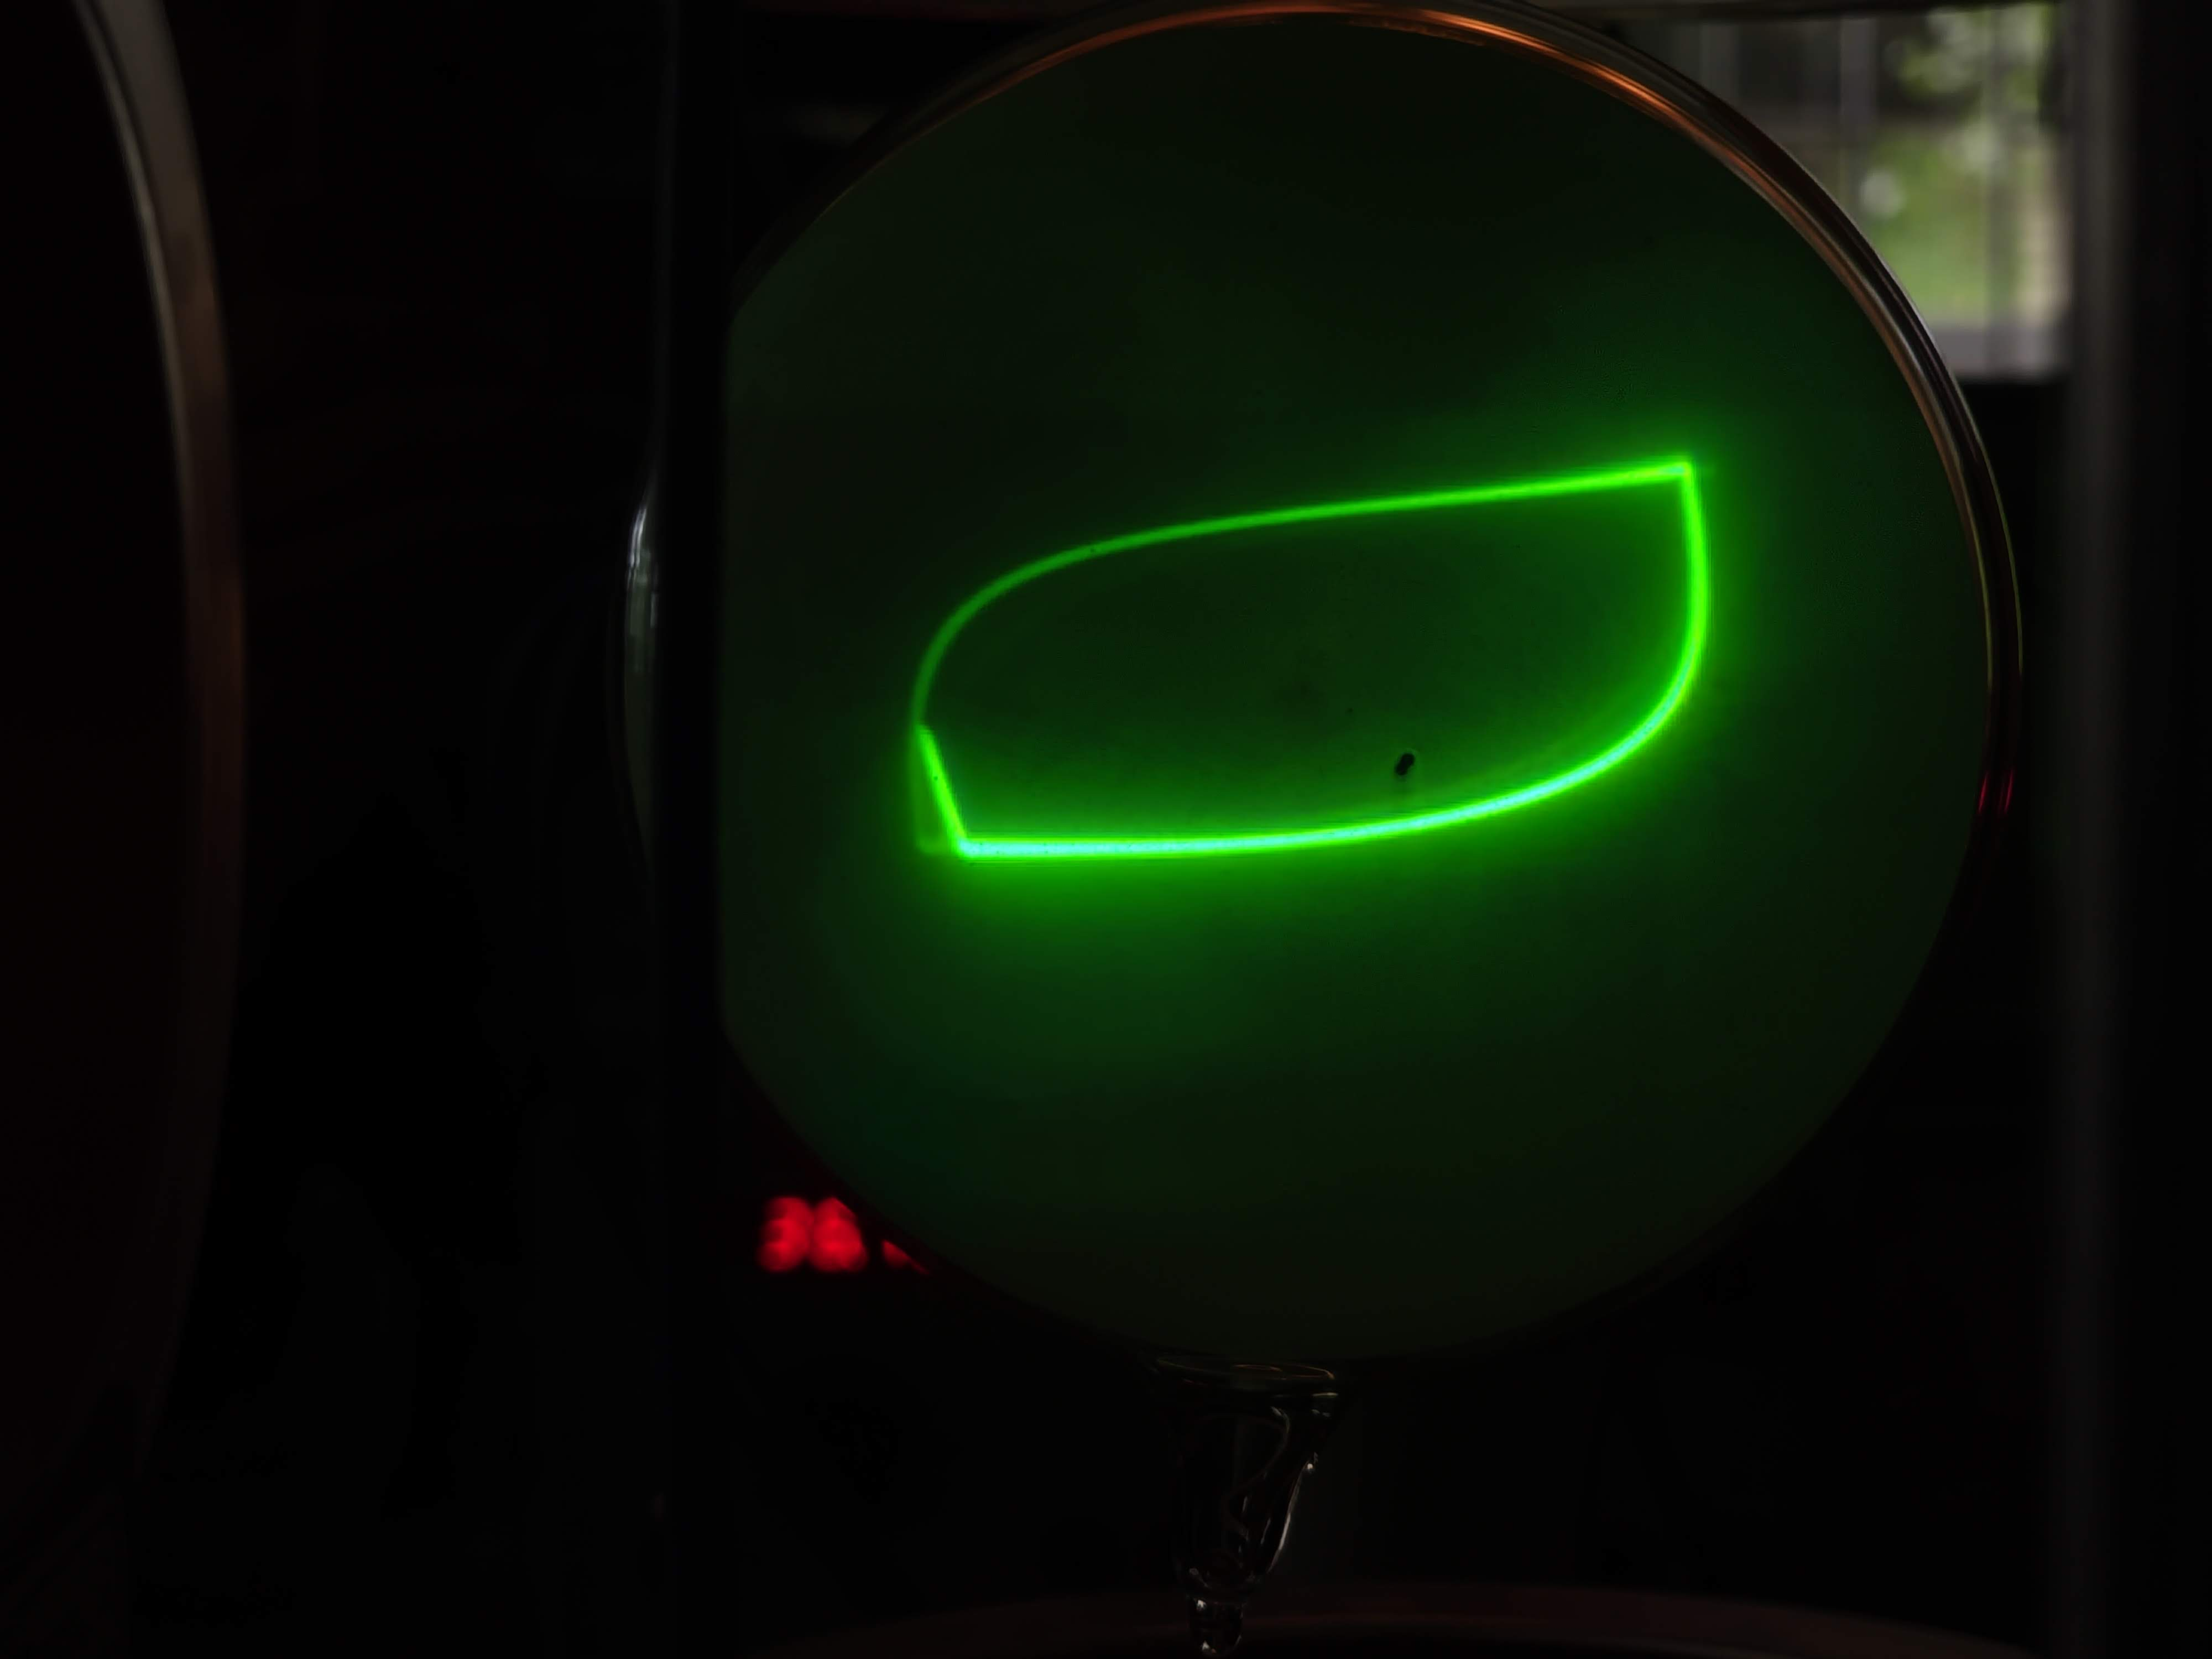
\includegraphics[width=\linewidth]{../Figures/liss-one.jpg}
		\label{fig:res_lissajous_circ}
	\end{subfigure}
	\hfill
	\begin{subfigure}{0.45\linewidth}
		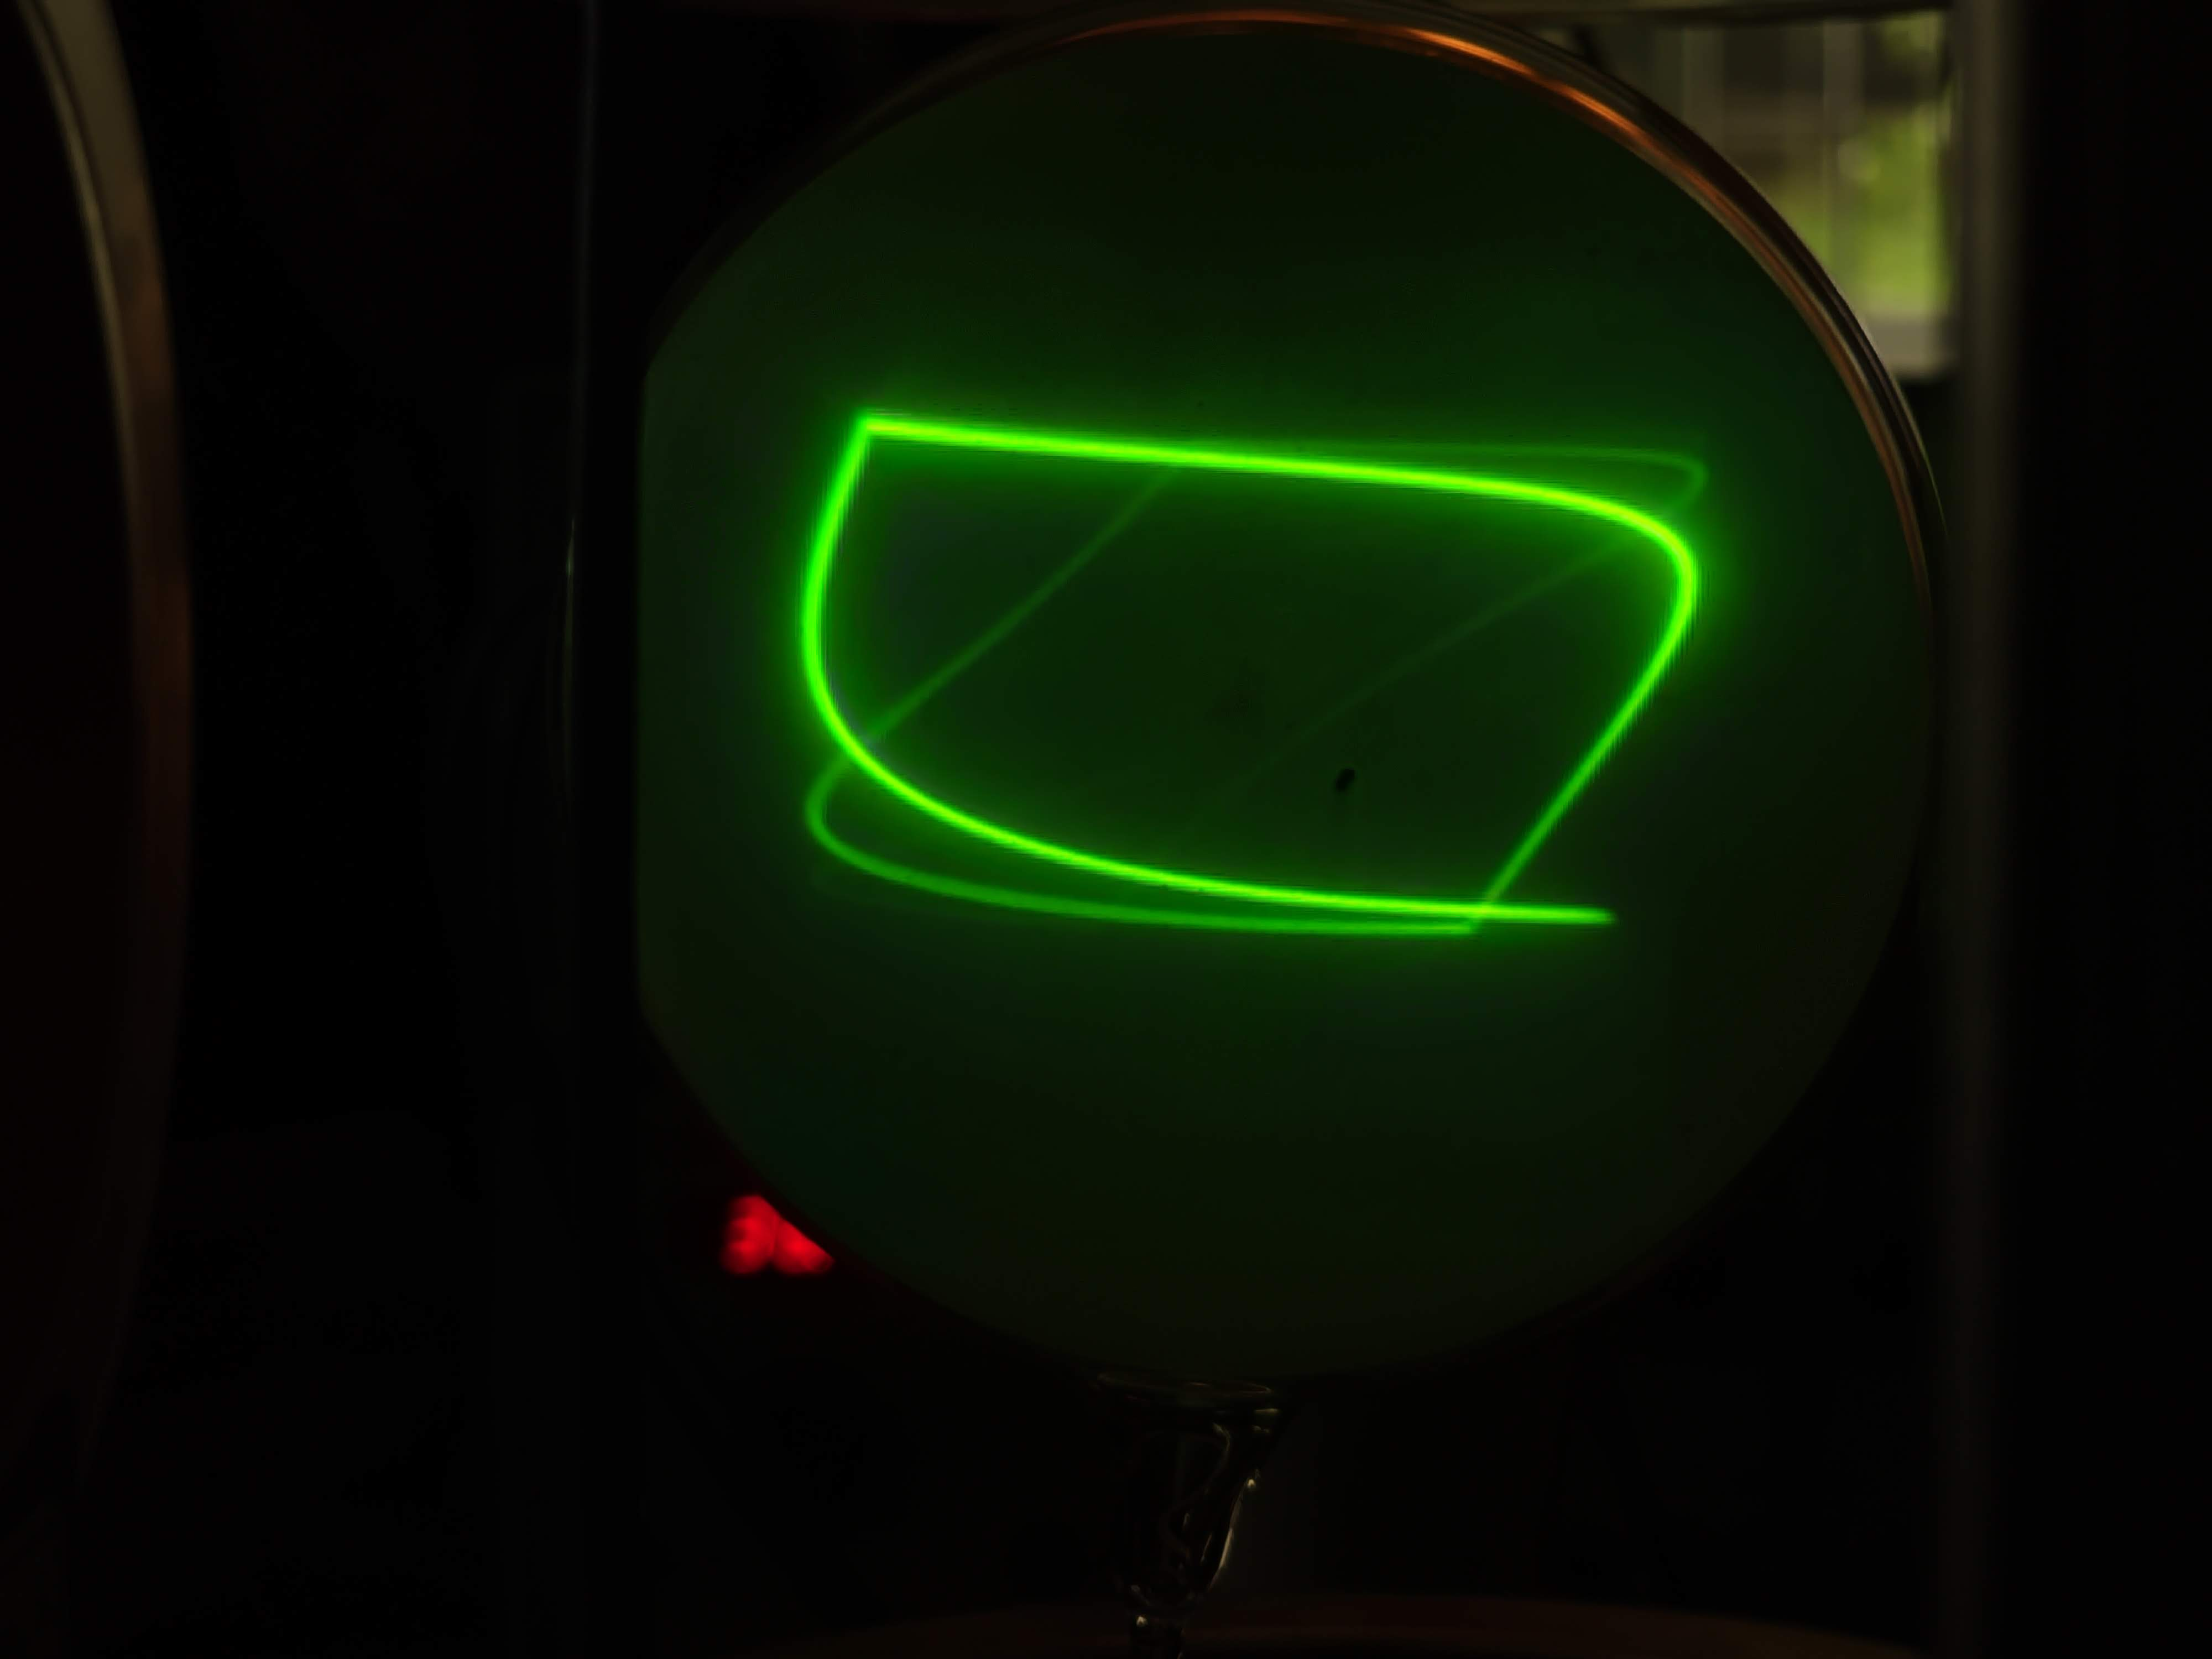
\includegraphics[width=\linewidth]{../Figures/liss-two.jpg}
		\label{fig:res_lissajous_2_1}
	\end{subfigure}
	\caption{Figuras de Lissajous observadas en la pantalla para diferentes
		razones de frecuencia y desfases entre las corrientes de los pares de
	bobinas en configuración Helmholtz.}
	\label{fig:resultados_lissajous}
\end{figure}

\section{Configuraciones de Campo de Gradiente (Anti-Helmholtz)}

En marcado contraste con la configuración anterior, los campos de
gradiente, generados por pares de bobinas en modo anti-Helmholtz,
produjeron patrones de naturaleza radial. El haz no trazaba una curva,
sino que convergía en un punto central y se expandía hacia afuera de forma
periódica. Se observó una \emph{pulsación rítmica} del haz, donde el radio
máximo del patrón circular en la pantalla era proporcional a la amplitud de
la corriente, mientras que la frecuencia de la pulsación coincidía con la
de la corriente de alimentación. Este comportamiento es la manifestación
visual directa del efecto de \emph{enfoque} (cuando el haz colapsa al
centro) y \emph{desenfoque} (cuando se expande) predicho por el modelo
cuadrupolar, confirmando la capacidad de dichos campos para manipular la
sección transversal del haz.

\begin{figure}[htbp!]
	\centering
	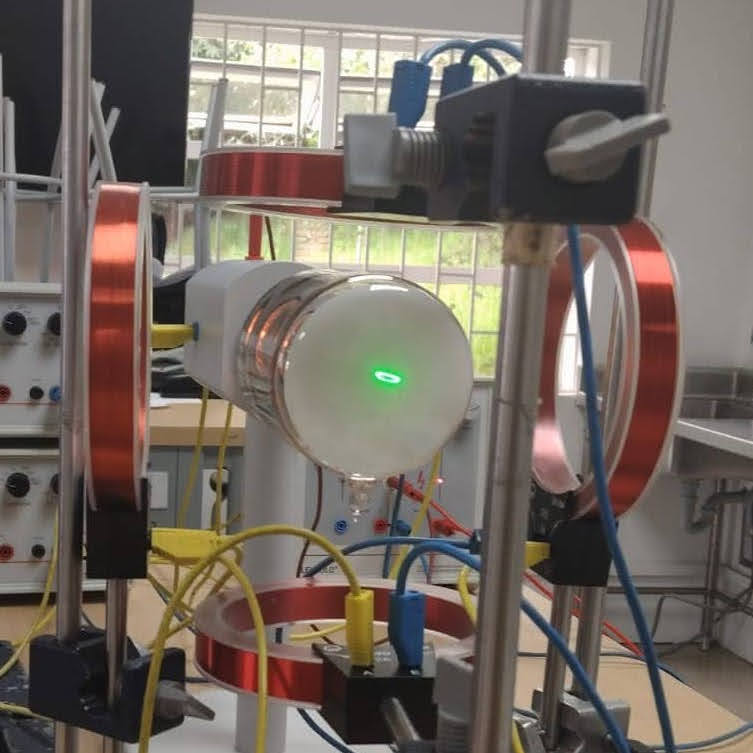
\includegraphics[width=0.6\linewidth]{../Figures/confienment.jpg}
	\caption{Patrón radial observado para la configuración anti-Helmholtz.}
	\label{fig:resultados_enfoque}
\end{figure}

\section{Configuración Mixta y Desdoblamiento del Haz}

Una configuración híbrida, empleando un par de bobinas en modo Helmholtz
(generando un campo relativamente uniforme en una dirección) y otro en modo
anti-Helmholtz (generando un campo de gradiente en la otra), produjo el
resultado más sorprendente. Se observó que el haz de electrones, en lugar
de trazar una curva o expandirse, se dividía y oscilaba de forma estable
entre dos posiciones discretas y bien definidas, como si la pantalla
presentara dos atractores estables para la trayectoria.

Este desdoblamiento del haz en dos puntos evoca, por su apariencia visual,
al patrón obtenido en el histórico experimento de Stern-Gerlach. No
obstante, es fundamental subrayar que la física subyacente \emph{no
corresponde} a una separación de estados de espín. Mientras que la
separación de espín es un fenómeno cuántico discreto dependiente de un
momento magnético intrínseco, el desdoblamiento observado aquí es de
naturaleza dinámica y puramente clásica. Se postula que la topología
compleja del campo magnético mixto crea un potencial con dos mínimos
locales, guiando al haz a saltar entre estas dos trayectorias estables a la
frecuencia de los campos. Dada la naturaleza no trivial de este resultado,
se posterga un análisis teórico detallado para la sección de \emph{Discusión}.

\begin{figure}[htbp!]
	\centering
	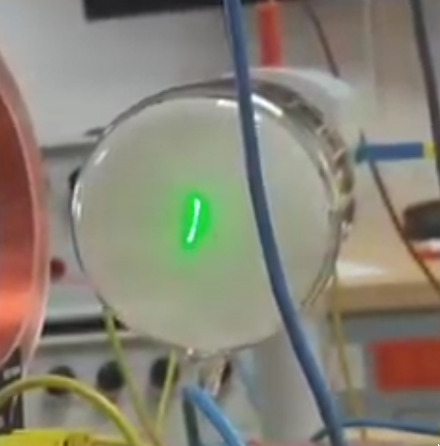
\includegraphics[width=0.7\linewidth]{../Figures/points.jpeg}
	\caption{Representación del desdoblamiento del haz observado con la
		configuración mixta. El punto luminoso del electrón oscila entre las
		dos posiciones estables (P1 y P2), un efecto clásico que recuerda
	visualmente al resultado de Stern-Gerlach.}
	\label{fig:resultados_desdoblamiento}
\end{figure}
